% Chapter Template

\chapter{The Logistic Map} % Main chapter title

\label{Chapter4} % Change X to a consecutive number; for referencing this chapter elsewhere, use \ref{ChapterX}

\lhead{Chapter 4. \emph{The Logistic Map}} % Change X to a consecutive number; this is for the header on each page - perhaps a shortened title
\section{The Map}
The logistic map is really simple. But as we have seen earlier with the Lorenz system earlier, simple maps can have very complicated dynamics. The logistic map is a one-dimensional map, and is defined by :-
\begin{equation}
	x_{n+1} = rx_n(1-x_n)
\end{equation}
where $r$ is a parameter. Note that this is the discrete version of the map, and a continuous description can also be defined similarly. This model is usually used to study population dynamics, so $r$ is referred to as the \textit{growth parameter}.

\section{Preliminary Numerics}
For all intents and purposes we shall restrict ourselves in the regime of $0<x\le 1$ and $0<r\le 4$. We shall see that this is the only interesting regime of parameters for this model. It is useful to think of $x$ as population to gain some physical intuition.

All the plots were made with initial condition $x=0.2$, and varying $r$.

First, let's look at what happens when $r\le1$. Fig. [\ref{fig:rle1}] plots the evolution for $r=0.1,0.5,1.0,1.1$. We see that for $r=0.1,0.5$, the population goes to zero pretty fast. When $r=1.0$, the population tends to go to zero as $n \rightarrow \infty$. On the other hand if $r$ is just above $1.0$, we see that there is a stable value to which the population converges to.

What does this tell us? It gives us the gloomy result that for low growth rates, the population of a certain species will go to zero at some point in time, ie. the species will become extinct.
\begin{figure}[h!]
	\centering
	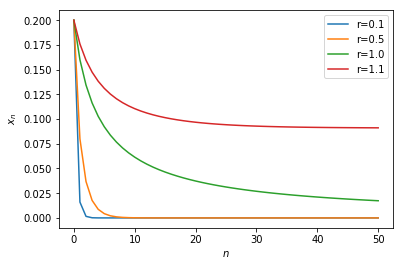
\includegraphics[scale=0.8]{Figures/rle1.png}
	\caption[An Electron]{$x_n$ vs $n$. We see that for $r<1$, $x_n$ goes to zero pretty fast.}
	\label{fig:rle1}
\end{figure}

Let's take a look at how the behaviour is for values of $r>1$ (Fig. [\ref{fig:rinbetween}]). For $r=2.8$, we see that the population oscillates a bit at the start and then settles down to a steady state value. But on the other hand, for $r=3.3$, the population just keeps oscillating periodically around the steady state value forever. This is where the logistic map becomes an important topic of study. One should note that the period of oscillations in rough $n=2$. 
\begin{figure}[h!]
	\centering
	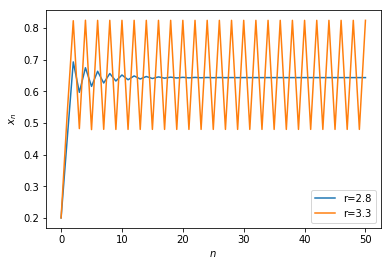
\includegraphics[scale=0.8]{Figures/rinbetween.png}
	\caption[An Electron]{$x_n$ vs $n$. For $r=2.8$, $x_n$ settles to a steady state value. For $r=3.3$, $x_n$ oscillates about the steady state.}
	\label{fig:rinbetween}
\end{figure}

Things really start getting interesting after $r=3.3$. For example, take a look at Fig. [\ref{fig:r38}], which plots the $x_n$ for $r=3.8$. We see that like $r=3.3$, $x_n$ oscillates around the steady state value, but now the period is not $n=2$! The period has now changed to a higher value. We could conjecture that for some value of the growth parameter, the period would really tend to infinity. This is a clear sign of chaos!

This is a really deep feature of the logistic map, which we shall hope to investigate further in this thesis, among other things.
\begin{figure}[h!]
	\centering
	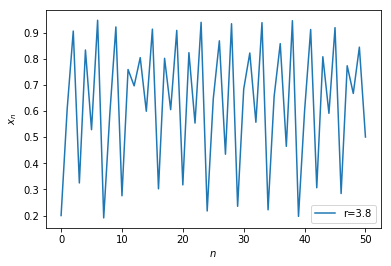
\includegraphics[scale=0.8]{Figures/r38.png}
	\caption[An Electron]{Numerical solutions for different initial conditions. Trajectories start to visibly diverge roughly around $t=30$.}
	\label{fig:r38}
\end{figure}